\setAuthor{Jaan Kalda}
\setRound{lahtine}
\setYear{2018}
\setNumber{G 9}
\setDifficulty{8}
\setTopic{Termodünaamika}

\prob{Õhkjahutus}
Valgusdiood tarbib elektrilist võimsust $P=\SI{50}W$. Dioodi jahutamiseks on see kinnitatud vaskplaadile paksusega $t=\SI{500}{\micro m}$. Vase soojusjuhtivustegur $k=\SI{385}{W/m.K}$. Juuresoleval graafikul on toodud plaadi temperatuur sõltuvuses vaadeldava punkti ja dioodi vahelise kauguse naturaallogaritmist. Kauguse mõõtmiseks kasutatud ühikud ei ole teada. Dioodi mõõtmed lugeda tühiselt väikseks. Milline on dioodi kasutegur (milline osa tarvitatud elektrienergiast kiirgub valgusenergiana)?

\textit{Märkus:} soojusjuhtivustegur on arvuliselt võrdne soojusenergiaga, mis kandub materjalis läbi ühikulise ristlõikepindala, kui temperatuur langeb ühe kraadi võrra ühe pikkusühiku kohta.
\begin{center}
	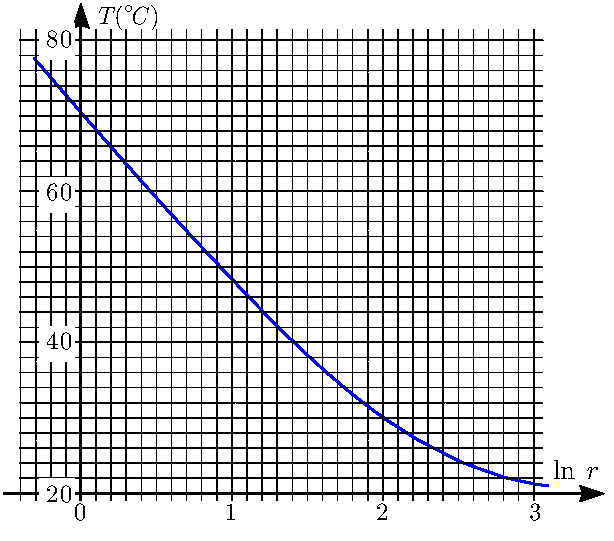
\includegraphics[width = 0.7\linewidth]{2018-lahg-09-yl.pdf}
\end{center}\hint
Piirkonnas, mis on dioodile lähedal pole mööda plaati leviv soojusenergia õhku jõudnud kaduda. Seal saab mugavalt dioodil eralduva soojusvõimsuse siduda piki plaati leviva soojusvooga vaadeldes dioodiga kontsentrilist silindrit raadiusega $r$ ning kõrgusega $t$.\solu
Piirkonnas, mis on dioodile lähedal ja kus seetõttu mööda plaati leviv soojusenergia pole veel jõudnud õhku kaduda, on soojusvoog leitav vaadeldes dioodiga kontsentrilist silindrid raadiusega $r$ ja kõrgusega $t$:
\[
P_s=2\pi rtk \frac{\mathrm d T}{\mathrm d r}=2\pi tk \frac{\mathrm d T}{\mathrm d \ln r},
\]
kus $P_s$ on soojusena dissipeeruv soojusvõimsus ning kasutasime $r^{-1}\dv*{T}{r} = \dv*{T}{\ln r}$. Näeme, et selles piirkonnas, kus antud eeldus kehtib, peab graafik olema sirgjoon ja selle tõus võrduma $\tan\alpha=2\pi tk$. Graafikul on väikeste $r$ väärtuste juures tõepoolest selline piirkond olemas ning graafiku puutuja tõus on seal $\tan\alpha\approx\SI{23.5}K$. Seega $P_s=kt\cdot \SI{23.5}K\approx \SI{28.5}W$. Kiiratud võimsus $P_k=P-P_s$ ning kasutegur $\eta=P_s/P\approx 0.43$.\probend